\chapter{Browser, HTTP, dan Network Internals}

\section*{Tujuan Pembelajaran}
\begin{itemize}
  \item Menjelaskan urutan peristiwa yang terjadi sejak sebuah alamat diketik
        sampai halaman tampil di layar, beserta biaya waktu tiap tahapnya.
  \item Membedakan HyperText Transfer Protocol (HTTP) versi 1.1, HTTP/2, dan
        HTTP/3 berdasarkan cara ketiganya menangani banyak permintaan
        sekaligus.
  \item Mengukur performa sebuah aplikasi web memakai \textit{browser DevTools}
        dan menetapkan angka \textit{baseline} yang dapat diuji ulang.
\end{itemize}

\section{Pendahuluan}

Aplikasi web yang lambat jarang disebabkan oleh satu masalah besar. Biasanya
penyebabnya adalah kumpulan keterlambatan kecil yang menumpuk. Ada waktu untuk
mencari alamat server. Ada waktu untuk membangun koneksi. Ada waktu tunggu
sampai byte pertama datang. Ada waktu untuk mengunduh berkas. Ada waktu untuk
menyusun tampilan. Setiap tahap itu punya biaya, dan biaya tersebut sering
tidak terlihat dari kode program.

Bab ini membahas tahap-tahap tersebut. Pembahasan dimulai dari cara browser
bekerja di dalam, lalu turun ke jaringan, lalu naik lagi ke proses menggambar
halaman. Tujuannya untuk membangun kemampuan menunjuk letak keterlambatan
secara tepat. Selain itu, bab ini juga bertujuan menjelaskan bahwa tanpa
pengukuran, optimasi tidak bisa akurat. Referensi utama yang digunakan adalah
spesifikasi resmi HTTP \cite{rfc9110} dan Grigorik \cite{grigorik2013hpbn}.

\section{Arsitektur Browser}

Browser modern bukan satu program tunggal, tetapi kumpulan proses yang berjalan
bersama dan saling berkirim pesan. Tugasnya terbagi, mulai dari mem-\textit{parse}
HyperText Markup Language (HTML) dan Cascading Style Sheets (CSS), mencari alamat
server lewat Domain Name System (DNS), sampai menggambar piksel memakai Graphics
Processing Unit (GPU). Gambar \ref{fig:proses-browser} menunjukkan susunannya,
dan Tabel \ref{tab:proses-browser} merangkum tugas tiap proses pada browser
berbasis Chromium.

\begin{figure}[!htb]
  \centering
  \begin{tikzpicture}[
    font=\scriptsize,
    proses/.style={draw, rounded corners, align=center, minimum height=0.95cm,
                   minimum width=2.3cm, fill=blue!8, font=\scriptsize\bfseries},
    utas/.style={draw, rounded corners, align=center, minimum height=0.85cm,
                 fill=orange!12, font=\scriptsize\bfseries},
    panah/.style={-{Stealth[length=1.8mm]}, gray!70, thick}
  ]
    \node[proses, fill=praditagreen!15, minimum width=5.2cm] (browser) at (0,0)
      {Proses Browser\\{\tiny\mdseries tab, address bar, profil}};

    \node[proses] (r1)   at (-4.85,-1.75) {Renderer 1};
    \node[proses] (r2)   at (-2.42,-1.75) {Renderer 2};
    \node[proses] (net)  at (0,-1.75)     {Network};
    \node[proses] (gpu)  at (2.42,-1.75)  {GPU};
    \node[proses] (util) at (4.85,-1.75)  {Utility};

    \foreach \n in {r1,r2,net,gpu,util}
      \draw[panah] (browser.south) -- (\n.north);

    \node[utas, minimum width=5.6cm] (main) at (-2.6,-3.9)
      {\textit{main thread}\\{\tiny\mdseries mem-\textit{parse} HTML, hitung
       \textit{style}, tata letak, gambar, jalankan JavaScript}};
    \node[utas, minimum width=4.4cm] (comp) at (3.1,-3.9)
      {compositor dan raster thread\\{\tiny\mdseries menggabungkan lapisan gambar}};

    \node[draw, dashed, gray, rounded corners, inner sep=7pt,
          fit=(main)(comp)] (kotak) {};
    \node[anchor=south west, font=\scriptsize\itshape, gray]
      at (kotak.north west) {Isi satu proses renderer};

    \draw[panah] (r1.south) -- ++(0,-0.55) -| (kotak.north west) ++(0,0);
  \end{tikzpicture}
  \caption{Susunan proses pada browser modern dan isi satu proses renderer}
  \label{fig:proses-browser}
\end{figure}

\begin{table}[!htb]
  \centering
  \caption{Proses utama pada browser modern dan tugasnya}
  \label{tab:proses-browser}
  \begin{tabularx}{\textwidth}{lX}
    \hline
    \textbf{Proses} & \textbf{Tugas} \\
    \hline
    Browser & Mengelola tab, address bar, menu, dan penyimpanan profil. \\
    \hline
    Renderer & Mem-\textit{parse} HTML dan CSS, menjalankan JavaScript, menggambar isi halaman. \\
    \hline
    Network & Menangani DNS, koneksi, dan seluruh lalu lintas HTTP. \\
    \hline
    GPU & Menggabungkan lapisan gambar untuk ditampilkan ke layar. \\
    \hline
    Utility & Menjalankan tugas terpisah seperti pemutaran audio dan video. \\
    \hline
  \end{tabularx}
\end{table}

Pemisahan proses ini menghasilkan dua konsekuensi. Pertama, satu tab
yang macet tidak mematikan seluruh browser, karena tab tersebut berjalan pada
proses \textit{renderer} sendiri. Kedua, halaman dari situs berlainan
dipisahkan ke proses tersendiri melalui mekanisme \textit{site isolation},
sehingga kode dari satu situs tidak dapat membaca memori situs lain.

Dua proses pada Tabel \ref{tab:proses-browser} sering tertukar, yaitu Renderer
dan GPU. Pembagiannya begini. Renderer menentukan \emph{apa} yang harus
digambar. Prosesnya mem-\textit{parse} HTML dan CSS, menghitung
\textit{style}, menghitung posisi tiap elemen, lalu menyusun daftar perintah
menggambar beserta pembagian lapisannya. GPU menjalankan \emph{bagaimana}
perintah itu diwujudkan menjadi piksel. Prosesnya menggambar tiap lapisan,
menggabungkannya, lalu menyerahkan hasilnya ke layar.

Analoginya seperti percetakan. Renderer adalah juru tata letak yang menentukan
teks, ukuran, dan posisi tiap kolom. GPU adalah mesin cetak yang mengubah
rancangan tersebut menjadi lembaran jadi. Pembagian ini juga menjelaskan dua hal
lain. Pertama, jumlah proses Renderer bertambah mengikuti situs yang dibuka,
sedangkan proses GPU cukup satu untuk seluruh browser. Kedua, kegagalan pada
driver kartu grafis hanya meng-\textit{crash} proses GPU. Browser tinggal menjalankan
ulang proses GPU tersebut, lalu meminta tiap Renderer menggambar ulang isinya.
Halaman berkedip sesaat, tetapi seluruh tab tetap terbuka dan isian form yang
belum dikirim tidak hilang.

Pertanyaan kemudian muncul: bagaimana bila banyak tab dibuka sekaligus? Satu
tab tidak selalu berarti satu proses. Chromium memakai aturan
\textit{process-per-site-instance}. Tab yang membuka situs sama umumnya berbagi
satu proses \textit{renderer}. Tab dari situs berlainan mendapat proses sendiri.
Iframe lintas situs juga dipindahkan ke proses terpisah, walaupun tampil di
dalam halaman yang sama. Gambar \ref{fig:tab-proses} menunjukkan contohnya.

\begin{figure}[!htb]
  \centering
  \begin{tikzpicture}[
    font=\scriptsize,
    tab/.style={draw, rounded corners=2pt, align=center, minimum height=0.95cm,
                minimum width=3.3cm, fill=praditagreen!12,
                font=\scriptsize\bfseries},
    ren/.style={draw, rounded corners, align=center, minimum height=1.05cm,
                minimum width=3.3cm, fill=blue!8, font=\scriptsize\bfseries},
    panah/.style={-{Stealth[length=1.8mm]}, gray!70, thick}
  ]
    \node[tab] (t1) at (-4.1,0) {Tab 1\\{\tiny\mdseries kampus.ac.id}};
    \node[tab] (t2) at (0,0)    {Tab 2\\{\tiny\mdseries kampus.ac.id/nilai}};
    \node[tab] (t3) at (4.1,0)  {Tab 3\\{\tiny\mdseries bank.co.id}};

    \node[ren] (r1) at (-4.1,-2.4) {Renderer 1\\{\tiny\mdseries kampus.ac.id}};
    \node[ren] (r3) at (0,-2.4)    {Renderer 3\\{\tiny\mdseries iklan.example}};
    \node[ren] (r2) at (4.1,-2.4)  {Renderer 2\\{\tiny\mdseries bank.co.id}};

    \draw[panah] (t1.south) -- (r1.north);
    \draw[panah] (t2.south) -- (r1.north east);
    \draw[panah] (t3.south) -- (r2.north);
    \draw[panah, dashed] (t1.south east) -- node[above right, font=\tiny\bfseries, gray]
      {iframe iklan} (r3.north west);
  \end{tikzpicture}
  \caption{Dua tab situs yang sama berbagi satu \textit{renderer}, sedangkan
           situs lain dan iframe lintas situs memperoleh proses sendiri}
  \label{fig:tab-proses}
\end{figure}

Aturan ini punya dua konsekuensi praktis. Pertama, jumlah tab yang banyak
menaikkan pemakaian memori secara nyata, karena tiap proses membawa \textit{copy}
mesin JavaScript dan struktur datanya sendiri. Kedua, tiap proses
\textit{renderer} punya \textit{main thread} sendiri, sehingga halaman berat di
satu tab tidak memperlambat tab lain, selama keduanya berasal dari situs yang
berbeda.

Bagian yang paling penting bagi pengembang aplikasi web adalah proses
\textit{renderer}. Di dalamnya terdapat satu utas utama yang disebut
\textit{main thread}. Utas tersebut mengerjakan hampir semua hal secara
bergantian: mem-\textit{parse} HTML, menghitung \textit{style}, menghitung tata
letak, menjalankan JavaScript, dan menanggapi klik pengguna. Hanya ada satu
utas untuk semua pekerjaan itu.

Analoginya seperti warung dengan satu kasir. Kasir tersebut melayani pesanan,
menghitung uang, membungkus makanan, dan menjawab pertanyaan pembeli. Selama
kasir sibuk menghitung pesanan besar, pembeli lain hanya bisa menunggu, meski
pesanan mereka sepele. Begitu pula \textit{main thread}. Selama sebuah fungsi
JavaScript berjalan lama, klik pengguna tidak diproses.

Dua contoh kasus nyata:

\begin{enumerate}
  \item Sebuah tabel menampilkan 5.000 baris data. Proses penyusunan baris
        memakan waktu 900 milidetik. Selama 900 milidetik itu, tombol
        \emph{cari} tidak bereaksi ketika diklik.
  \item Sebuah halaman mem-\textit{parse} berkas JavaScript Object Notation
        (JSON) berukuran 8 MB memakai \texttt{JSON.parse}. Proses
        \textit{parsing} tidak dapat dipotong di tengah jalan, sehingga halaman
        membeku sampai proses tersebut selesai.
\end{enumerate}

\section{DNS, TCP, dan TLS}

Sebelum satu byte HTML terkirim, tiga urusan harus diselesaikan lebih dahulu.
Alamat server harus ditemukan lewat DNS. Koneksi harus dibangun lewat
Transmission Control Protocol (TCP). Kanal aman harus disepakati lewat
Transport Layer Security (TLS). Gambar \ref{fig:koneksi} menunjukkan urutannya.

\begin{figure}[ht]
  \centering
  \begin{tikzpicture}[
    node distance=0.6cm and 0.5cm,
    tahap/.style={draw, rounded corners, minimum height=1cm, minimum width=2.1cm,
                  align=center, font=\footnotesize\bfseries},
    panah/.style={-{Stealth[length=2mm]}, thick}
  ]
    \node[tahap, fill=blue!8]  (dns)  {DNS\\1 RTT};
    \node[tahap, fill=blue!8,  right=of dns]  (tcp)  {TCP\\1 RTT};
    \node[tahap, fill=blue!8,  right=of tcp]  (tls)  {TLS 1.3\\1 RTT};
    \node[tahap, fill=green!10, right=of tls] (req)  {Request\\terkirim};
    \node[tahap, fill=orange!12, right=of req] (ttfb) {Byte pertama\\tiba};

    \draw[panah] (dns) -- (tcp);
    \draw[panah] (tcp) -- (tls);
    \draw[panah] (tls) -- (req);
    \draw[panah] (req) -- (ttfb);
  \end{tikzpicture}
  \caption{Tahap sebelum byte pertama halaman tiba di browser. Tiap tahap
           menghabiskan satu RTT (\textit{round trip time})}
  \label{fig:koneksi}
\end{figure}

\textbf{DNS} menerjemahkan nama domain menjadi alamat Internet Protocol
(IP).
Browser bertanya ke \textit{resolver}, lalu \textit{resolver} menelusuri
berjenjang sampai menemukan server yang memegang jawabannya. Hasilnya disimpan
sementara selama masa TTL (\textit{Time To Live}) pada beberapa tingkat, yaitu
\textit{cache} browser, \textit{cache} sistem operasi, dan \textit{cache}
\textit{resolver}. Analoginya seperti mencari nomor kontak di buku alamat
sebelum menelepon. Nomor yang sudah pernah dicatat tidak perlu dicari lagi.
Contohnya, kunjungan pertama ke sebuah domain menuntut pencarian penuh,
sedangkan kunjungan berikutnya memakai \textit{cache} sehingga biayanya nyaris
nol. Contoh lain, sebuah situs akademik dipindahkan dari server lama di pusat
data kampus ke server baru di penyedia \textit{cloud}, sehingga alamat IP-nya
berubah. TTL yang pendek, misalnya 60 detik, membuat pengguna beralih ke alamat
baru dalam hitungan menit. TTL yang panjang, misalnya 24 jam, membuat sebagian
pengguna masih diarahkan ke server lama sampai sehari penuh. Sebaliknya, TTL
pendek menambah jumlah pencarian DNS pada hari-hari biasa.

\textbf{TCP} menyediakan aliran byte yang urut dan andal di atas jaringan yang
tidak andal. Koneksi dibuka lewat \textit{three-way handshake}, yaitu tiga
pesan berurutan. Browser mengirim SYN (\textit{synchronize}) sebagai permintaan
membuka koneksi. Server membalas SYN-ACK, yaitu persetujuan sekaligus
permintaan balik. Browser menutupnya dengan ACK (\textit{acknowledge}) sebagai
tanda siap. Analoginya seperti membuka percakapan telepon: "halo", "halo, ya",
lalu "baik, saya mulai". Ketiga pesan itu menghabiskan satu RTT. Setelah
koneksi terbuka, paket yang hilang dikirim ulang, dan urutannya dirapikan
kembali sebelum diserahkan ke aplikasi.

\textbf{TLS} mengurus dua hal: memastikan lawan bicara memang server yang
dituju, dan menjaga isi percakapan tidak terbaca pihak lain. Server mengirim
sertifikat, browser memeriksa rantai sertifikat tersebut sampai ke
\textit{Certificate Authority} (CA) yang dipercaya, lalu kedua pihak menyepakati
kunci sesi. Analoginya seperti memeriksa kartu identitas lebih dahulu, baru
kemudian bertukar surat di dalam amplop tersegel. Contohnya, sertifikat yang
kedaluwarsa membuat browser menolak melanjutkan koneksi. Contoh lain, sesi yang
pernah terjadi dapat dilanjutkan lewat \textit{session resumption}, sehingga
pembukaan berikutnya lebih singkat.

Istilah RTT adalah singkatan dari \textit{round trip time}, yaitu waktu yang
dibutuhkan sebuah paket untuk pergi ke server dan kembali lagi. Angka ini
ditentukan oleh jarak fisik dan kualitas jaringan, bukan oleh kecepatan
program. Server yang cepat sekalipun tidak dapat memperpendek RTT.

Penyebabnya terlihat begitu jalur yang dilewati sebuah paket dirinci. Paket
tidak melompat langsung dari browser ke server. Paket harus melewati modem atau
router di sisi pengguna, jaringan akses milik penyedia internet, titik
pertukaran trafik, kabel serat optik darat, kabel laut bila tujuannya lintas
negara, jaringan penyedia di negara tujuan, lalu perangkat di dalam pusat data.
Tiap perangkat perantara membaca alamat tujuan, menentukan jalur berikutnya,
dan sering menahan paket sebentar di antrean. Satu lintasan seperti ini biasa
melewati belasan sampai puluhan perangkat.

Batas bawahnya ditentukan fisika. Cahaya di dalam serat optik merambat sekitar
200.000 km per detik. Jarak Jakarta ke Frankfurt kira-kira 11.000 km, sehingga
sekali jalan butuh sekitar 55 milidetik dan pulang pergi sekitar 110 milidetik.
Angka nyata pada Tabel \ref{tab:rtt} lebih besar, yaitu 190 milidetik, karena
kabel tidak terbentang lurus dan tiap perangkat perantara menambah waktu
tunggu. Bandingkan dengan Jakarta ke Singapura yang berjarak sekitar 900 km.
Batas fisikanya hanya sekitar 9 milidetik, dan angka nyatanya 35 milidetik.

Tabel \ref{tab:rtt} menunjukkan dampaknya. Perhitungannya memakai tiga RTT
sebelum permintaan terkirim, sesuai Gambar \ref{fig:koneksi}.

\begin{table}[!htb]
  \centering
  \caption{Biaya pembukaan koneksi pada jarak yang berbeda, sebelum server
           mengerjakan apa pun}
  \label{tab:rtt}
  \begin{tabularx}{\textwidth}{lXrr}
    \hline
    \textbf{Lokasi server} & \textbf{Contoh} & \textbf{RTT} & \textbf{3 RTT} \\
    \hline
    Satu kota      & Jakarta ke Jakarta      & 10 ms  & 30 ms  \\
    \hline
    Regional       & Jakarta ke Singapura    & 35 ms  & 105 ms \\
    \hline
    Antarbenua     & Jakarta ke Frankfurt    & 190 ms & 570 ms \\
    \hline
  \end{tabularx}
\end{table}

Angka pada kolom terakhir terjadi sebelum server mengerjakan apa pun. Server
dengan waktu proses 20 milidetik tetap terasa lambat bila diakses lintas benua.
Inilah alasan Content Delivery Network (CDN) ditempatkan dekat pengguna, dan
alasan koneksi yang sudah terbuka sebaiknya dipakai ulang.

Cara kerja CDN sederhana. Penyedia CDN menempatkan server titipan di banyak
kota, termasuk Jakarta dan Singapura. Server titipan itu disebut \textit{edge
server}, sedangkan server asli milik aplikasi disebut \textit{origin}. Nama
domain aplikasi diarahkan ke jaringan CDN, sehingga permintaan pengguna mendarat
di \textit{edge server} terdekat, bukan langsung ke \textit{origin}. Bila \textit{copy}
berkas yang diminta sudah ada di sana, berkas langsung dikirim. Bila belum ada,
\textit{edge server} mengambilnya sekali ke \textit{origin}, menyimpannya, lalu
melayani permintaan berikutnya dari \textit{copy} tersebut.

Analoginya seperti gudang cabang. Pembeli di Jakarta tidak perlu memesan
langsung ke pabrik di Jerman, karena barang yang sama sudah dititipkan di gudang
Jakarta. Contohnya, gambar dan berkas CSS dari server Frankfurt yang tadinya
menuntut RTT 190 milidetik cukup diambil dari Jakarta dengan RTT 10 milidetik.
Contoh lain, halaman yang isinya berubah tiap detik tetap harus diambil dari
\textit{origin}, sehingga manfaat CDN untuk halaman semacam itu terbatas pada
pemendekan jarak koneksi saja.

Beberapa cara menekan biaya ini:

\begin{itemize}
  \item Koneksi dipakai ulang untuk banyak permintaan, bukan dibuka dan ditutup
        berulang kali.
  \item \texttt{preconnect} dipasang untuk domain pihak ketiga yang pasti
        dipakai, sehingga koneksi dibangun lebih awal.
  \item TLS 1.3 \cite{rfc8446} dipakai, karena \textit{handshake} nya lebih pendek
        dibanding TLS 1.2.
  \item Jumlah domain berbeda dalam satu halaman dibatasi, karena tiap domain
        baru menuntut rangkaian DNS, TCP, dan TLS sendiri.
\end{itemize}

Istilah domain pihak ketiga pada butir di atas perlu diperjelas. Yang dimaksud
adalah domain di luar domain aplikasi itu sendiri. Contohnya penyedia huruf
seperti \texttt{fonts.gstatic.com}, CDN gambar, layanan analitik, peta, atau
\textit{gateway} pembayaran. Tiap domain semacam itu menuntut rangkaian DNS,
TCP, dan TLS sendiri, karena koneksi ke domain aplikasi tidak dapat dipakai
ulang untuk domain lain.

Penanda \texttt{preconnect} meminta browser membuka rangkaian tersebut lebih
awal, yaitu saat HTML masih di-\textit{parse}, jauh sebelum aset benar-benar
diminta. Ketika giliran aset itu tiba, koneksinya sudah siap. Penanda ini
dipasang hanya untuk domain yang pasti dipakai, karena koneksi yang dibuka
tetapi tidak terpakai justru memboroskan sumber daya. Listing
\ref{lst:preconnect} menunjukkan penulisannya.

\begin{lstlisting}[language=html, caption={Membuka koneksi ke domain pihak ketiga lebih awal, tersedia di \berkas{sources/chapter02/preconnect.html}}, label={lst:preconnect}]
<!-- Koneksi lengkap: DNS, TCP, dan TLS -->
<link rel="preconnect" href="https://fonts.gstatic.com" crossorigin>

<!-- Hanya pencarian DNS, dipakai bila aset belum tentu diminta -->
<link rel="dns-prefetch" href="https://cdn.contoh.ac.id">
\end{lstlisting}

Listing \ref{lst:curl} memperlihatkan biaya tiap tahap secara langsung.

\begin{lstlisting}[language=bash, caption={Mengukur waktu tiap tahap koneksi, format keluarannya di \berkas{sources/chapter02/format-curl.txt}}, label={lst:curl}]
# Format keluaran disimpan di berkas agar perintahnya pendek dan mudah disalin.
curl -o /dev/null -s -w @format-curl.txt https://www.pradita.ac.id/

# Keluarannya:
# dns:0.009726s tcp:0.033991s tls:0.084639s ttfb:0.338771s total:0.342899s versi:HTTP/2
\end{lstlisting}

Isi \texttt{format-curl.txt} beserta skrip pembungkusnya tersedia pada
\berkas{sources/chapter02/}. Skrip \texttt{ukur-koneksi.sh} menjalankan perintah
tersebut berulang kali sekaligus menghitung durasi tiap tahap. Perlu diperhatikan,
angka \texttt{curl} bersifat kumulatif sejak permintaan dimulai, sehingga durasi
tiap tahap diperoleh dengan pengurangan. Perhatikan pula bahwa
\texttt{pradita.ac.id} tanpa \texttt{www} menjawab dengan pengalihan 301,
sehingga pengukuran sebaiknya langsung memakai alamat tujuannya.

\section{HTTP/1.1, HTTP/2, dan HTTP/3}

Ketiga versi HTTP memindahkan data yang sama, dan semantiknya dijabarkan pada
dokumen Request for Comments (RFC) 9110 \cite{rfc9110}. Perbedaannya terletak pada cara banyak permintaan
dilayani dalam satu waktu. Perbedaan itu yang menentukan performa halaman
dengan puluhan aset.

\subsection*{HTTP/1.1}

Satu koneksi melayani satu permintaan pada satu waktu. Permintaan berikutnya
menunggu sampai respons sebelumnya selesai. Gejala ini disebut
\textit{head-of-line blocking}. Browser menyiasatinya dengan membuka sekitar
enam koneksi paralel per domain, dan tiap koneksi menanggung biaya pembukaan
sendiri. Gambar \ref{fig:http1} menggambarkan pola tersebut. Misalkan sebuah
halaman meminta empat berkas sekaligus, yaitu A berupa \texttt{style.css}, B
berupa \texttt{app.js}, C berupa \texttt{logo.png}, dan D berupa
\texttt{foto.jpg}. Lebar tiap kotak menggambarkan lama pengunduhannya.

Analoginya seperti loket pembayaran uang kuliah dengan enam jendela. Satu
mahasiswa dengan berkas bermasalah menahan seluruh antrean di jendelanya,
walaupun jendela lain tetap berjalan.

\begin{figure}[!htb]
  \centering
  \begin{tikzpicture}[
    font=\small,
    blok/.style={draw, minimum height=0.62cm, anchor=west, align=center,
                 font=\small\bfseries},
    setup/.style={blok, fill=orange!25, minimum width=2.8cm},
    baris/.style={anchor=east, font=\small\bfseries},
    ket/.style={anchor=west, font=\footnotesize, gray},
    sumbu/.style={-{Stealth[length=2mm]}, gray}
  ]
    \node[baris, font=\footnotesize] at (-0.15,0)    {Koneksi 1};
    \node[baris, font=\footnotesize] at (-0.15,-0.8) {Koneksi 2};
    \node[baris, font=\footnotesize] at (-0.15,-1.6) {Koneksi 3};

    \node[setup] at (0,0)    {DNS+TCP+TLS};
    \node[setup] at (0,-0.8) {DNS+TCP+TLS};
    \node[setup] at (0,-1.6) {DNS+TCP+TLS};

    \node[blok, minimum width=1.9cm, fill=blue!25]  at (2.8,0)    {A};
    \node[blok, minimum width=1.6cm, fill=blue!12]  at (4.7,0)    {D};
    \node[blok, minimum width=2.6cm, fill=red!22]   at (2.8,-0.8) {B};
    \node[blok, minimum width=1.5cm, fill=green!25] at (2.8,-1.6) {C};

    \node[ket] at (6.45,0) {D menunggu A selesai};

    \draw[sumbu] (0,-2.25) -- (8.6,-2.25)
      node[anchor=north east, font=\footnotesize] {waktu};
  \end{tikzpicture}
  \caption{HTTP/1.1 membuka koneksi terpisah untuk tiap permintaan yang berjalan
           bersamaan, dan permintaan berikutnya pada satu koneksi menunggu
           giliran. A: \texttt{style.css}, B: \texttt{app.js},
           C: \texttt{logo.png}, D: \texttt{foto.jpg}. Lebar kotak
           menggambarkan lama pengunduhan}
  \label{fig:http1}
\end{figure}

\subsection*{HTTP/2}

HTTP/2 \cite{rfc9113} memecah data menjadi \textit{frame} biner, lalu \textit{frame}
dari banyak permintaan
diselang-seling dalam satu koneksi. Cara ini disebut \textit{multiplexing}.
Header juga di-\textit{compress} memakai HPACK \cite{rfc7541}. Nama HPACK bukan
singkatan berhuruf awal, melainkan berasal dari \textit{header packing}, dan
judul resmi spesifikasinya adalah \textit{HPACK: Header Compression for
HTTP/2}. Cara kerjanya memakai dua tabel. Tabel statis berisi header yang lazim
dipakai, misalnya \texttt{:method: GET}. Tabel dinamis berisi header yang sudah
pernah dikirim pada koneksi tersebut. Header yang berulang cukup dikirim sebagai
nomor indeks, bukan sebagai teks penuh, dan sisanya dipadatkan dengan pengodean
Huffman. Hasilnya, permintaan berulang tidak lagi membawa header yang sama
berkali-kali.

Gambar \ref{fig:http2} menunjukkan hasilnya. Kembali ke analogi loket. Berkas
setiap mahasiswa dipotong menjadi lembaran kecil, lalu petugas memproses
lembaran itu bergantian. Tidak ada satu berkas yang menahan berkas lain sampai
selesai. Meski begitu, karena semua \textit{frame} berjalan di atas satu
koneksi TCP, satu paket yang hilang menahan seluruh koneksi sampai paket
tersebut dikirim ulang.

\begin{figure}[!htb]
  \centering
  \begin{tikzpicture}[
    font=\small,
    blok/.style={draw, minimum height=0.62cm, anchor=west, align=center,
                 font=\small\bfseries},
    setup/.style={blok, fill=orange!25, minimum width=2.8cm},
    baris/.style={anchor=east, font=\small\bfseries},
    ket/.style={anchor=west, font=\footnotesize, gray},
    sumbu/.style={-{Stealth[length=2mm]}, gray}
  ]
    \node[baris, font=\footnotesize] at (-0.15,0) {Koneksi 1};
    \node[setup] at (0,0) {DNS+TCP+TLS};

    \foreach \i/\w/\t in {0/blue!25/A, 1/red!22/B, 2/green!25/C, 3/blue!25/A,
                          4/red!22/B, 5/green!25/C, 6/blue!25/A, 7/red!22/B} {
      \pgfmathsetmacro{\x}{2.8 + \i*0.66}
      \node[blok, minimum width=0.64cm, fill=\w] at (\x,0) {\t};
    }

    \node[ket, font=\footnotesize] at (0,-1.0)
      {\textit{frame} milik A, B, dan C diselang-seling di atas satu koneksi};

    \draw[sumbu] (0,-1.6) -- (8.6,-1.6)
      node[anchor=north east, font=\footnotesize] {waktu};
  \end{tikzpicture}
  \caption{HTTP/2 memotong tiap permintaan menjadi \textit{frame}, lalu
           menyelang-nyelingnya di atas satu koneksi. A: \texttt{style.css},
           B: \texttt{app.js}, C: \texttt{logo.png}}
  \label{fig:http2}
\end{figure}

\subsection*{HTTP/3}

HTTP/3 \cite{rfc9114} berjalan di atas QUIC \cite{rfc9000}, dan QUIC memakai
User Datagram Protocol (UDP). Nama QUIC awalnya merupakan singkatan dari
\textit{Quick UDP Internet Connections} pada versi rancangan Google. Sejak
distandarkan pada RFC 9000, QUIC diperlakukan sebagai nama, bukan singkatan.
Gambar \ref{fig:http3} menggambarkan perbedaannya dengan HTTP/2.

Perbedaan itu berakar pada cara tiap versi menangani paket yang hilang. TCP
menyerahkan data ke aplikasi secara urut. Ketika satu paket hilang, seluruh
paket yang tiba sesudahnya ditahan di \textit{buffer} sampai paket tersebut
selesai dikirim ulang, karena TCP tidak tahu paket itu milik permintaan yang
mana. Pada HTTP/1.1, penahanan tersebut hanya menyangkut satu koneksi, dan
permintaan lain di koneksi berbeda tetap berjalan. Pada HTTP/2, seluruh permintaan justru
berbagi satu koneksi TCP, sehingga satu paket yang hilang menahan
\textit{frame} milik semua permintaan sekaligus. Gejala ini disebut
\textit{head-of-line blocking} di tingkat TCP.

QUIC memindahkan pencatatan urutan dari tingkat koneksi ke tingkat aliran.
Tiap aliran punya nomor urut dan \textit{buffer} sendiri, dan QUIC mengetahui
tiap paket milik aliran yang mana. Paket yang hilang pada aliran B hanya menahan
aliran B, sedangkan aliran A dan C tetap diserahkan ke browser. Pada Gambar
\ref{fig:http3}, hal ini terlihat dari kotak X di aliran B yang tidak
menghentikan barisan kotak A dan C.
Header di-\textit{compress} memakai QPACK \cite{rfc9204}, yaitu penyesuaian HPACK untuk
QUIC. Judul resmi spesifikasinya adalah \textit{QPACK: Field Compression for
HTTP/3}. Penyesuaian itu diperlukan karena aliran QUIC dapat tiba tidak
berurutan, sedangkan tabel dinamis HPACK menuntut urutan yang pasti. QUIC juga
memangkas jumlah RTT saat koneksi dibuka. Pada HTTP/2, pembukaan koneksi
berjalan dua tahap terpisah, yaitu \textit{handshake} TCP selama satu RTT, lalu
\textit{handshake} TLS selama satu RTT lagi. QUIC menyatukan keduanya dalam satu
pertukaran pesan, sehingga koneksi baru cukup satu RTT. Untuk server yang pernah
dikunjungi, QUIC bahkan dapat mengirim permintaan bersamaan dengan pesan
pembuka, yang disebut mode 0-RTT. Tabel \ref{tab:http-versi} merangkum perbedaan
ketiga versi tersebut.

\begin{figure}[!htb]
  \centering
  \begin{tikzpicture}[
    font=\small,
    blok/.style={draw, minimum height=0.62cm, anchor=west, align=center,
                 font=\small\bfseries},
    setup/.style={blok, fill=orange!25, minimum width=2.8cm},
    baris/.style={anchor=east, font=\small\bfseries},
    ket/.style={anchor=west, font=\footnotesize, gray},
    sumbu/.style={-{Stealth[length=2mm]}, gray}
  ]
    \node[baris, font=\footnotesize] at (-0.15,0)    {Aliran A};
    \node[baris, font=\footnotesize] at (-0.15,-0.8) {Aliran B};
    \node[baris, font=\footnotesize] at (-0.15,-1.6) {Aliran C};

    \node[setup, minimum height=2.22cm, minimum width=2.4cm, align=center]
      at (0,-0.8) {QUIC\\\textit{handshake}};

    \foreach \i in {0,1,2,3,4} {
      \pgfmathsetmacro{\x}{2.6 + \i*0.72}
      \node[blok, minimum width=0.7cm, fill=blue!25] at (\x,0) {A};
      \node[blok, minimum width=0.7cm, fill=green!25] at (\x,-1.6) {C};
    }

    \node[blok, minimum width=0.7cm, fill=red!22]  at (2.6,-0.8)  {B};
    \node[blok, minimum width=0.7cm, fill=gray!35] at (3.32,-0.8) {X};
    \node[blok, minimum width=0.7cm, fill=red!22]  at (4.76,-0.8) {B};
    \node[blok, minimum width=0.7cm, fill=red!22]  at (5.48,-0.8) {B};

    \node[ket] at (6.3,-0.8) {X: paket hilang};
    \node[ket] at (6.3,-1.6) {A dan C tetap jalan};

    \draw[sumbu] (0,-2.25) -- (8.6,-2.25)
      node[anchor=north east, font=\footnotesize] {waktu};
  \end{tikzpicture}
  \caption{HTTP/3 memisahkan tiap permintaan menjadi aliran mandiri, sehingga
           paket yang hilang pada satu aliran tidak menahan aliran lain.
           A: \texttt{style.css}, B: \texttt{app.js}, C: \texttt{logo.png},
           X: paket yang hilang}
  \label{fig:http3}
\end{figure}

\begin{table}[!htb]
  \centering
  \caption{Ringkasan perbedaan tiga versi HTTP}
  \label{tab:http-versi}
  \begin{tabularx}{\textwidth}{lXXX}
    \hline
     & \textbf{HTTP/1.1} & \textbf{HTTP/2} & \textbf{HTTP/3} \\
    \hline
    Format & Teks & Biner & Biner \\
    \hline
    Transport & TCP & TCP & QUIC di atas UDP \\
    \hline
    Permintaan sekaligus & Satu per koneksi & Banyak, diselang-seling & Banyak, aliran mandiri \\
    \hline
    Blocking & Di tingkat permintaan & Di tingkat TCP & Hanya pada aliran terdampak \\
    \hline
    Header & Dikirim penuh & Di-\textit{compress} HPACK & Di-\textit{compress} QPACK \\
    \hline
    Pindah jaringan & Koneksi putus & Koneksi putus & Berlanjut lewat \textit{connection ID} \\
    \hline
  \end{tabularx}
\end{table}

Dua contoh dampaknya di lapangan:

\begin{enumerate}
  \item Halaman katalog dengan 80 gambar kecil. Pada HTTP/1.1, gambar diambil
        enam per waktu dan sisanya mengantre. Pada HTTP/2, seluruh permintaan
        berjalan di satu koneksi, dan waktu muat turun tajam.
  \item Pengguna berpindah dari Wi-Fi kampus ke jaringan seluler saat mengunggah
        berkas. Pada HTTP/2, koneksi dikenali dari pasangan alamat IP dan nomor
        port di kedua sisi. Begitu alamat IP berubah, pasangan itu ikut berubah,
        koneksi dianggap putus, dan unggahan diulang dari awal. Pada HTTP/3,
        koneksi dikenali dari \textit{connection ID}, yaitu nomor pengenal yang
        disepakati saat koneksi dibuka dan tidak bergantung pada alamat IP.
        Server mencocokkan paket yang datang berdasarkan nomor tersebut, lalu
        melanjutkan unggahan yang sedang berjalan.
\end{enumerate}

Perlu dicatat, HTTP/2 dan HTTP/3 tidak membuat jumlah aset menjadi tidak
penting. Aset di sini berarti seluruh berkas yang diminta browser untuk
menyusun satu halaman, di luar dokumen HTML-nya sendiri. Contohnya berkas CSS,
berkas JavaScript, gambar, huruf, ikon, dan berkas video. Halaman katalog
sederhana saja mudah memuat lebih dari seratus aset. Setiap aset tetap menuntut
permintaan, \textit{parsing}, dan pemakaian memori.

\section{Siklus Hidup Request dan Event Loop}

Setelah respons tiba, pekerjaan berpindah ke \textit{main thread}. Utas
tersebut diatur oleh \textit{event loop}. Cara kerjanya berulang dan sederhana:
ambil satu tugas dari antrean, jalankan sampai selesai, kosongkan antrean
\textit{microtask}, lalu beri kesempatan browser menggambar ulang layar. Gambar
\ref{fig:event-loop} menunjukkan satu putarannya.

Ada dua jenis antrean yang dilayani \textit{main thread}. Pertama, antrean
tugas atau \textit{task queue}, yang isinya sering disebut \textit{macrotask}.
Kedua, antrean \textit{microtask}. Keduanya dilayani utas yang sama, tetapi
dengan aturan pengambilan yang berbeda.

Istilah tugas atau \textit{macrotask} berarti satu satuan pekerjaan yang
dititipkan ke antrean untuk dijalankan \textit{main thread}. Contohnya
menjalankan skrip yang baru selesai diunduh, menanggapi klik atau ketikan
pengguna, menjalankan fungsi yang dijadwalkan lewat \texttt{setTimeout},
memproses respons \texttt{fetch} yang sudah tiba, dan menangani pesan dari
\textit{web worker}. Isi antrean umumnya berupa eksekusi kode JavaScript, tetapi
tidak selalu. Melanjutkan \textit{parsing} HTML yang tiba bertahap dari jaringan
juga dijalankan sebagai tugas, dan pekerjaan itu tetap memakai \textit{main
thread} walaupun tidak ada satu baris JavaScript pun yang berjalan. Perlu dicatat, spesifikasi HTML mengizinkan lebih dari satu
\textit{task queue}, dipisah menurut sumbernya, misalnya antrean \textit{timer}
dan antrean \textit{event}. Browser memilih satu tugas dari salah satu antrean
tersebut pada tiap putaran.

\textit{Microtask} adalah pekerjaan kecil yang menumpang di sela dua
\textit{macrotask}. Antreannya hanya satu.
Isinya hampir selalu lanjutan dari \textit{promise}, yaitu badan \texttt{.then}
dan baris setelah \texttt{await}. Bedanya dengan tugas biasa ada pada waktu
eksekusinya. Setelah satu tugas selesai, \textbf{seluruh} antrean
\textit{microtask} dikosongkan lebih dahulu, termasuk \textit{microtask} baru
yang lahir di tengah proses itu, dan baru setelah itu browser boleh menggambar
ulang layar serta mengambil tugas berikutnya. Aturan itu menjaga urutan
\textit{promise} tetap terduga, tetapi juga berarti rantai \textit{promise}
yang tidak habis-habis dapat menahan penggambaran layar. Tabel
\ref{tab:antrean} merangkum perbedaan perlakuan kedua antrean tersebut, dan
Listing \ref{lst:urutan} membuktikan urutannya lewat contoh kode.

\begin{table}[!htb]
  \centering
  \caption{Perbedaan perlakuan antrean \textit{macrotask} dan \textit{microtask}}
  \label{tab:antrean}
  \begin{tabularx}{\textwidth}{lXX}
    \hline
     & \textbf{\textit{Task queue} (\textit{macrotask})} & \textbf{Antrean \textit{microtask}} \\
    \hline
    Jumlah antrean & Boleh lebih dari satu, dipisah per sumber & Hanya satu \\
    \hline
    Diambil tiap putaran & Satu tugas saja & Dikosongkan seluruhnya \\
    \hline
    Pekerjaan baru saat berjalan & Menunggu putaran berikutnya & Ikut dikerjakan pada putaran yang sama \\
    \hline
    Penggambaran layar & Boleh terjadi sesudahnya & Ditahan sampai antrean kosong \\
    \hline
  \end{tabularx}
\end{table}

Pertanyaan kemudian muncul: apakah JavaScript dikerjakan lebih dahulu, lalu
penggambaran menyusul, atau keduanya bagian dari proses yang sama? Jawabannya,
penggambaran layar adalah salah satu tahap di dalam putaran \textit{event loop}
itu sendiri, dan tahap tersebut memakai \textit{main thread} yang sama dengan
JavaScript. Urutan satu putaran lengkapnya: ambil satu \textit{macrotask} dan
jalankan sampai selesai, kosongkan antrean \textit{microtask}, lalu masuk tahap
penggambaran berupa \textit{callback} \texttt{requestAnimationFrame},
perhitungan \textit{style}, perhitungan tata letak, penggambaran, dan penyusunan
lapisan.

Dua hal perlu ditegaskan. Pertama, tahap penggambaran tidak dijalankan pada
tiap putaran. Browser hanya menggambar mengikuti laju \textit{refresh} layar, umumnya
60 kali per detik, sehingga jatahnya sekitar 16,7 milidetik per \textit{frame}.
Bila tidak ada yang berubah, tahap itu dilewati. Kedua, karena berbagi satu
utas, JavaScript dan penggambaran saling menahan. Tugas yang berjalan 200
milidetik membuat browser melewatkan sekitar dua belas kesempatan menggambar,
dan animasi pun tersendat. Satu-satunya bagian yang benar-benar terpisah adalah
penggabungan lapisan di proses GPU, dan itulah sebabnya animasi
\texttt{transform} serta \texttt{opacity} tetap mulus walaupun \textit{main
thread} sedang sibuk.

\begin{lstlisting}[language=TypeScript, caption={Urutan eksekusi tugas dan \textit{microtask}, tersedia di \berkas{sources/chapter02/urutan-event-loop.js}}, label={lst:urutan}]
console.log("1: kode sinkron");
setTimeout(() => console.log("4: tugas berikutnya"), 0);
Promise.resolve().then(() => console.log("3: microtask"));
console.log("2: kode sinkron");
// Keluaran berurutan: 1, 2, 3, 4.
// Baris 3 tetap lebih dulu daripada baris 4, walaupun tundaan setTimeout 0 ms.
\end{lstlisting}

\begin{figure}[ht]
  \centering
  \begin{tikzpicture}[
    node distance=0.55cm and 0.9cm,
    kotak/.style={draw, rounded corners, minimum height=0.9cm, minimum width=2.6cm,
                  align=center, font=\footnotesize\bfseries},
    panah/.style={-{Stealth[length=2mm]}, thick}
  ]
    \node[kotak, minimum width=3cm, fill=blue!8] (task)
      {Ambil satu \textit{macrotask}\\dari antrean tugas};
    \node[kotak, minimum width=3cm, fill=blue!8, right=of task] (jalan)
      {Jalankan sampai\\selesai};
    \node[kotak, minimum width=3cm, fill=orange!12, right=of jalan] (micro)
      {Kosongkan antrean\\\textit{microtask}};
    \node[kotak, minimum width=3cm, fill=green!10, below=1.1cm of micro] (render)
      {Hitung \textit{style},\\tata letak, gambar};

    \draw[panah] (task) -- (jalan);
    \draw[panah] (jalan) -- (micro);
    \draw[panah] (micro) -- (render);
    \draw[panah] (render) -| ([xshift=-1.6cm]task.west) -- (task.west);
  \end{tikzpicture}
  \caption{Satu putaran \textit{event loop} pada \textit{main thread}}
  \label{fig:event-loop}
\end{figure}

Kunci pemahamannya ada pada kalimat \emph{jalankan sampai selesai}. Sebuah
tugas tidak dapat dipotong di tengah. Selama tugas berjalan, tidak ada
penggambaran ulang dan tidak ada tanggapan atas klik. Tugas yang berjalan lebih
dari 50 milidetik disebut \textit{long task}, dan itulah sumber utama
antarmuka yang terasa berat. Listing \ref{lst:longtask} memberi satu
contohnya.

\begin{lstlisting}[language=TypeScript, caption={Tugas berat yang menahan seluruh antarmuka, tersedia di \berkas{sources/chapter02/tugas-berat.ts}}, label={lst:longtask}]
function hitungTotal(pesanan: Pesanan[]): number {
  let total = 0;
  // Perulangan panjang ini menahan main thread sampai selesai.
  for (const item of pesanan) {
    total += hitungPajakBerlapis(item); // proses berat per item
  }
  return total;
}
\end{lstlisting}

Dua cara umum mengatasinya:

\begin{enumerate}
  \item Pekerjaan dipecah menjadi potongan kecil, lalu dijadwalkan bertahap
        memakai \texttt{setTimeout} atau \texttt{scheduler.yield}. Antarmuka
        mendapat celah untuk menanggapi klik di sela potongan tersebut.
  \item Pekerjaan dipindahkan ke \textit{web worker}, yang berjalan pada utas
        terpisah. Cara ini cocok untuk \textit{parsing} data besar dan perhitungan
        berat.
\end{enumerate}

\section{Rendering Pipeline dan Critical Rendering Path}

Halaman tidak langsung tampil setelah HTML tiba. Ada rangkaian tahap yang harus
dilalui, dan rangkaian itu disebut \textit{critical rendering path}. HTML
diubah menjadi DOM (\textit{Document Object Model}), sedangkan CSS diubah
menjadi CSSOM (\textit{CSS Object Model}). Keduanya lalu dipadukan. Gambar
\ref{fig:crp} menunjukkan urutan tahapnya.

\begin{figure}[ht]
  \centering
  \begin{tikzpicture}[
    node distance=0.45cm and 0.45cm,
    tahap/.style={draw, rounded corners, minimum height=0.85cm, minimum width=1.75cm,
                  align=center, font=\scriptsize\bfseries},
    panah/.style={-{Stealth[length=2mm]}, thick}
  ]
    \node[tahap, fill=blue!8] (html) {HTML\\$\rightarrow$ DOM};
    \node[tahap, fill=blue!8, below=of html] (css) {CSS\\$\rightarrow$ CSSOM};
    \node[tahap, fill=orange!12, right=1.1cm of $(html)!0.5!(css)$] (tree) {Render\\Tree};
    \node[tahap, fill=orange!12, right=of tree] (layout) {Layout};
    \node[tahap, fill=orange!12, right=of layout] (paint) {Paint};
    \node[tahap, fill=green!10, right=of paint] (comp) {Composite};

    \draw[panah] (html) -- (tree);
    \draw[panah] (css) -- (tree);
    \draw[panah] (tree) -- (layout);
    \draw[panah] (layout) -- (paint);
    \draw[panah] (paint) -- (comp);
  \end{tikzpicture}
  \caption{Tahap penyusunan halaman dari berkas mentah sampai piksel di layar}
  \label{fig:crp}
\end{figure}

Penjelasan tiap tahap memakai analogi penyusunan koran kampus. DOM adalah
naskah berita yang sudah diketik. CSSOM adalah panduan \textit{style} berisi
ukuran huruf dan lebar kolom. Render tree
adalah naskah yang sudah dipadukan dengan panduan \textit{style}, tanpa bagian
yang memang tidak dicetak. Layout adalah penentuan posisi
tiap elemen di halaman. Paint adalah proses menggambar isi tiap kotak.
Composite adalah penggabungan lapisan menjadi satu halaman utuh.

Dua hal menghambat rangkaian ini:

\begin{enumerate}
  \item \textbf{CSS bersifat \textit{render blocking}.} Halaman tidak digambar
        sebelum seluruh CSS diunduh dan di-\textit{parse}. Berkas CSS berukuran 400 KB
        pada jaringan lambat menahan tampilan meski HTML sudah siap.
  \item \textbf{Script tanpa penanda bersifat \textit{parser blocking}.} Tag
        \texttt{script} biasa di dalam \texttt{head} menghentikan \textit{parsing}
        HTML sampai berkas selesai diunduh dan dijalankan.
\end{enumerate}

\begin{lstlisting}[language=html, caption={Script yang menahan \textit{parsing} dan perbaikannya, tersedia di \berkas{sources/chapter02/defer-async.html}}, label={lst:defer}]
<!-- Menahan parsing HTML sampai analytics.js selesai dijalankan -->
<script src="/js/analytics.js"></script>

<!-- Diunduh paralel dengan parsing HTML, dijalankan setelah parsing selesai -->
<script src="/js/analytics.js" defer></script>

<!-- Diunduh paralel juga, tetapi langsung dijalankan begitu unduhan selesai -->
<script src="/js/iklan.js" async></script>
\end{lstlisting}

Kata paralel di sini berarti pengunduhan berjalan bersamaan dengan
\textit{parsing} HTML, bukan menggantikannya. Browser tetap membaca HTML dari
atas ke bawah, sedangkan berkas skrip diambil di latar belakang. Beda
\texttt{defer} dan \texttt{async} ada pada waktu eksekusinya. Skrip
\texttt{defer} baru dijalankan setelah \textit{parsing} selesai, dan bila ada
beberapa, urutannya mengikuti urutan penulisan di HTML. Skrip \texttt{async}
dijalankan begitu unduhannya selesai, sehingga urutannya tidak dapat
diandalkan, dan eksekusinya masih dapat memotong \textit{parsing}. Karena itu
\texttt{defer} dipakai untuk skrip aplikasi yang saling bergantung, sedangkan
\texttt{async} dipakai untuk skrip yang berdiri sendiri, misalnya pengukur
kunjungan. Perbandingan ketiganya ada pada Listing \ref{lst:defer}.

Pertanyaan berikutnya, siapa yang mengerjakan tahap-tahap tersebut. Jawabannya
terbagi antara beberapa proses dan utas, mengikuti pembagian pada Seksi 2.2.
Tabel \ref{tab:penanggung-jawab-render} merangkumnya.

\begin{table}[!htb]
  \centering
  \caption{Penanggung jawab tiap tahap penggambaran halaman}
  \label{tab:penanggung-jawab-render}
  \begin{tabularx}{\textwidth}{Xl}
    \hline
    \textbf{Tahap} & \textbf{Penanggung jawab} \\
    \hline
    Menghitung \textit{style}, menghitung tata letak, merekam perintah menggambar & Renderer, \textit{main thread} \\
    \hline
    Membagi halaman menjadi lapisan, menangani \textit{scroll} dan animasi \texttt{transform} & Renderer, \textit{compositor thread} \\
    \hline
    Mengubah perintah menggambar menjadi piksel & Renderer, \textit{raster thread}, dibantu GPU \\
    \hline
    Menggabungkan lapisan lalu menampilkannya ke layar & Proses GPU \\
    \hline
    Menggambar antarmuka browser, misalnya tab dan address bar & Proses Browser \\
    \hline
  \end{tabularx}
\end{table}

Dua baris pertama pada tabel tersebut menjelaskan hampir seluruh masalah
performa tampilan. Baris pertama berbagi utas dengan JavaScript, sehingga tugas
yang berat langsung menahan perhitungan \textit{style} dan tata letak. Baris
kedua berjalan pada utas terpisah, sehingga \textit{scroll} biasanya tetap
lancar walaupun \textit{main thread} sedang sibuk. Begitu animasi menyentuh
properti yang mengubah tata letak, pekerjaannya kembali ke \textit{main thread},
dan kemulusannya hilang.

Perubahan tampilan setelah halaman tampil juga punya biaya berbeda. Mengubah
lebar sebuah elemen memaksa perhitungan tata letak ulang, lalu penggambaran
ulang. Mengubah \texttt{transform} atau \texttt{opacity} hanya menyentuh tahap
\textit{composite}, sehingga jauh lebih murah. Animasi yang halus memanfaatkan
sifat ini.

\section{Core Web Vitals}

Pengukuran perlu angka yang disepakati. Core Web Vitals \cite{webdev-vitals}
adalah tiga metrik yang mewakili tiga pertanyaan pengguna. LCP
(\textit{Largest Contentful Paint}) mengukur waktu sampai elemen isi terbesar
tampil. INP (\textit{Interaction to Next Paint}) mengukur jeda antara interaksi
pengguna dan pembaruan tampilan berikutnya. CLS (\textit{Cumulative Layout
Shift}) mengukur seberapa banyak tata letak bergeser tanpa diminta pengguna.
Tabel \ref{tab:cwv} merangkum ambang batasnya.

\begin{table}[!htb]
  \centering
  \caption{Core Web Vitals dan ambang batasnya}
  \label{tab:cwv}
  \begin{tabularx}{\textwidth}{lXll}
    \hline
    \textbf{Metrik} & \textbf{Pertanyaan pengguna} & \textbf{Baik} & \textbf{Buruk} \\
    \hline
    LCP & Kapan isi utama terlihat?      & $\leq$ 2,5 detik & $>$ 4 detik \\
    \hline
    INP & Seberapa cepat halaman menanggapi? & $\leq$ 200 ms & $>$ 500 ms \\
    \hline
    CLS & Apakah tata letak melompat?    & $\leq$ 0,1 & $>$ 0,25 \\
    \hline
  \end{tabularx}
\end{table}

Contoh untuk LCP:

\begin{enumerate}
  \item Pada halaman detail produk, elemen terbesar biasanya foto produk. LCP
        ditentukan oleh waktu foto tersebut tampil.
  \item Pada halaman artikel tanpa gambar, elemen terbesar adalah blok
        paragraf pembuka. LCP ditentukan oleh waktu teks tersebut tampil,
        sehingga pemuatan \textit{font} ikut berpengaruh.
\end{enumerate}

INP mengukur interaksi di dalam halaman yang sama, bukan perpindahan ke halaman
baru. Interaksi yang dihitung hanya tiga jenis, yaitu klik, ketukan layar
sentuh, dan penekanan tombol keyboard. \textit{Scroll} dan \textit{hover} tidak
ikut dihitung. Yang diukur adalah jeda sejak pengguna menekan sampai layar
benar-benar berubah, dan jeda tersebut terdiri atas tiga bagian seperti pada
Tabel \ref{tab:inp}.

\begin{table}[!htb]
  \centering
  \caption{Tiga bagian penyusun jeda yang diukur INP}
  \label{tab:inp}
  \begin{tabularx}{\textwidth}{lX}
    \hline
    \textbf{Bagian} & \textbf{Isinya} \\
    \hline
    \textit{Input delay} & Menunggu \textit{main thread} bebas dari tugas yang sedang berjalan \\
    \hline
    \textit{Processing time} & Menjalankan \textit{event handler} milik aplikasi \\
    \hline
    \textit{Presentation delay} & Menghitung \textit{style} dan tata letak, menggambar, sampai \textit{frame} baru tampil \\
    \hline
  \end{tabularx}
\end{table}

Contoh untuk INP:

\begin{enumerate}
  \item Halaman jadwal kuliah menyembunyikan satu bagian lalu menampilkan
        bagian lain setelah tombol tab ditekan. Seluruh rangkaiannya, mulai
        dari penekanan tombol sampai bagian baru tampil, dihitung sebagai satu
        interaksi.
  \item Tombol \emph{filter} pada halaman katalog ditekan ketika sebuah tugas
        selama 300 milidetik sedang berjalan. \textit{Event handler} belum
        dapat berjalan sama sekali, sehingga angka INP sudah buruk sejak
        bagian \textit{input delay}, walaupun isi \textit{handler} tersebut
        hanya satu baris.
\end{enumerate}

Perlu dicatat, INP sebuah halaman bukan rata-rata seluruh interaksi, melainkan
interaksi terburuk. Pada halaman dengan interaksi sangat banyak, sebagian kecil
interaksi terburuk diabaikan, tetapi maknanya tetap sama, yaitu INP mewakili
pengalaman terjelek, bukan pengalaman yang khas.

Berbeda dengan LCP dan INP yang dibaca dalam satuan waktu, CLS tidak punya
satuan. Nilainya berupa skor polos, karena disusun dari dua pecahan yang
sama-sama relatif terhadap ukuran layar. Skor satu pergeseran dihitung dengan
mengalikan \textit{impact fraction}, yaitu bagian layar yang terpengaruh elemen
yang bergeser, dengan \textit{distance fraction}, yaitu jarak pergeseran dibagi
dimensi layar terbesar. Misalnya sebuah blok menempati 50 persen tinggi layar
lalu terdorong ke bawah sejauh 25 persen tinggi layar. Skornya 0,5 dikali 0,25
sama dengan 0,125, dan angka itu saja sudah melewati ambang baik yang bernilai
0,1. CLS sebuah halaman adalah jumlah skor pergeseran pada rentang waktu
terburuk selama kunjungan.

Contoh untuk CLS:

\begin{enumerate}
  \item Banner pengumuman disisipkan di atas konten setelah halaman tampil.
        Seluruh isi terdorong ke bawah, dan pengguna salah menekan tautan.
  \item Gambar dimuat tanpa atribut \texttt{width} dan \texttt{height}. Ruang
        untuk gambar baru terbentuk saat gambar tiba, sehingga teks di
        bawahnya bergeser.
\end{enumerate}

Satu catatan penting soal cara membaca angka. Nilai yang dipakai adalah
persentil ke-75 dari pengguna nyata, bukan rata-rata. Artinya begini. Seluruh
kunjungan diurutkan dari yang paling cepat sampai yang paling lambat, lalu
diambil nilai pada urutan 75 persen. Nilai itu berarti 75 persen kunjungan
sama cepat atau lebih cepat daripadanya, sedangkan 25 persen sisanya lebih
lambat. Jadi yang dipakai bukan 25 persen tercepat, melainkan batas yang masih
menanggung seperempat pengguna paling lambat.

Contohnya, sebuah halaman diakses 100 kali dalam sehari. Angka LCP dari seluruh
kunjungan diurutkan, lalu diambil kunjungan ke-75. Bila nilainya 2,4 detik,
halaman tersebut lolos ambang LCP, walaupun 25 kunjungan sisanya bisa jadi
mencapai 5 detik. Rata-rata tidak dipakai karena mudah tertutupi. Sembilan
puluh kunjungan dari perangkat cepat dengan LCP 1 detik akan menutupi sepuluh
kunjungan dari perangkat lambat dengan LCP 8 detik, dan rata-ratanya tetap
terlihat bagus di angka 1,7 detik. Kelompok yang lambat itulah yang justru
paling perlu diperbaiki.

Pengukuran di komputer pengembang disebut \textit{lab data}, dan hasilnya
hampir selalu lebih baik daripada kenyataan.

\section{Penguasaan Browser DevTools}

Semua konsep di atas dapat dilihat langsung memakai DevTools. Tabel
\ref{tab:devtools} merangkum panel yang paling sering dipakai.

\begin{table}[!htb]
  \centering
  \caption{Panel DevTools dan kegunaannya}
  \label{tab:devtools}
  \begin{tabularx}{\textwidth}{lX}
    \hline
    \textbf{Panel} & \textbf{Kegunaan} \\
    \hline
    Network & Melihat urutan permintaan, ukuran berkas, dan rincian waktu tiap tahap. \\
    \hline
    Performance & Melihat pekerjaan \textit{main thread} dan menemukan \textit{long task}. \\
    \hline
    Lighthouse \cite{lighthouse} & Menjalankan audit performa dan aksesibilitas secara otomatis. \\
    \hline
    Coverage & Menghitung berapa persen CSS dan JavaScript yang benar-benar terpakai. \\
    \hline
  \end{tabularx}
\end{table}

Pada panel Network, kolom \textit{waterfall} memecah waktu satu permintaan
menjadi beberapa bagian. Bagian \emph{Queueing} dan \emph{Stalled} menandakan
permintaan menunggu giliran koneksi. Bagian \emph{DNS Lookup},
\emph{Initial connection}, dan \emph{SSL} (\textit{Secure Sockets Layer}, nama lama TLS) sesuai dengan
tahap pada Gambar
\ref{fig:koneksi}. Bagian \emph{Waiting} adalah waktu tunggu respons server,
yang lebih dikenal sebagai Time To First Byte (TTFB). Bagian \emph{Content Download} adalah waktu
pengunduhan isi.

Cara membacanya sederhana. Bila bagian \emph{Waiting} yang panjang, masalahnya
ada di server atau basis data. Bila bagian \emph{Content Download} yang
panjang, masalahnya ada pada ukuran berkas. Bila bagian \emph{Queueing} yang
panjang, jumlah permintaan serentak terlalu banyak.

Pengukuran wajib dilakukan dengan \textit{throttling} yang mendekati kondisi pengguna.
Aktifkan \textit{network throttling} pada profil Slow 4G. Aktifkan juga \textit{throttling} Central Processing Unit (CPU) pada faktor
4 kali lebih lambat. Tanpa \textit{throttling} itu,
hasil pengukuran hanya menggambarkan komputer pengembang, bukan ponsel
mahasiswa.

\section{Ringkasan}

Browser modern berjalan sebagai banyak proses, tetapi hampir seluruh pekerjaan
satu halaman ditanggung oleh satu \textit{main thread} di dalam proses
Renderer. Sebelum halaman itu bahkan mulai diminta, DNS, TCP, dan TLS sudah
menghabiskan waktu tersendiri, dan besarnya ditentukan oleh jarak fisik serta
jumlah perangkat yang dilewati paket, bukan oleh kecepatan program di server.

Ketiga versi HTTP menangani beban itu dengan cara berbeda. HTTP/1.1 melayani
satu permintaan per koneksi, sehingga browser terpaksa membuka banyak koneksi
sekaligus. HTTP/2 menyelang-nyeling \textit{frame} milik banyak permintaan di
atas satu koneksi. HTTP/3 memisahkan tiap permintaan menjadi aliran mandiri,
sehingga satu paket yang hilang tidak lagi menahan permintaan lain.

Setelah respons tiba, giliran \textit{main thread} yang menjadi penentu. Tugas
JavaScript berjalan sampai selesai tanpa dapat dipotong, sehingga tugas panjang
membuat antarmuka berhenti menanggapi. Penggambaran layar pun bukan proses
terpisah, melainkan salah satu tahap dalam putaran \textit{event loop} yang
sama. Di sisi berkas, CSS menahan penggambaran, dan skrip tanpa \texttt{defer}
menahan \textit{parsing} HTML.

Seluruh gejala tersebut diringkas oleh Core Web Vitals menjadi tiga angka yang
mewakili pengalaman pengguna, dan angka itu dibaca pada persentil ke-75 agar
pengguna dengan perangkat lambat tidak tertutupi. Pesan terakhirnya paling
penting: optimasi tanpa \textit{baseline} tidak dapat dibuktikan, sehingga
pengukuran selalu didahulukan.

\section{Latihan}

Seluruh skrip yang dipakai pada latihan ini tersedia di
\berkas{sources/chapter02/}, dihitung relatif terhadap akar repositori.

\subsection*{Latihan 1: Profiling dan Penetapan Baseline Performa}

Latihan ini memakai dua halaman situs kampus sebagai objek pengukuran, yaitu
halaman depan \url{https://www.pradita.ac.id} dan satu halaman dalam
\url{https://www.pradita.ac.id/praktisi-akademisi}. Hasil akhirnya adalah catatan angka awal beserta
kondisi pengukurannya.

Satu batasan dipegang sejak awal. Seluruh pengukuran di sini bersifat mengamati,
bukan membebani. Pengukuran dilakukan sebagai satu pengguna biasa memakai
browser dan permintaan tunggal. Uji beban dengan banyak pengguna tiruan,
misalnya memakai k6 seperti pada Listing \ref{lst:k6}, hanya boleh dijalankan
pada sistem milik sendiri atau setelah memperoleh izin tertulis dari pengelola
sistem. Menjalankannya tanpa izin pada situs produksi mengganggu layanan dan
dapat dianggap serangan.

\begin{enumerate}
  \item Buka \texttt{https://www.pradita.ac.id} pada jendela penyamaran, agar
        ekstensi dan \textit{cache} lama tidak memengaruhi hasil.
  \item Buka DevTools, aktifkan Slow 4G dan \textit{throttling} CPU 4 kali lebih lambat,
        lalu muat ulang halaman dengan \textit{cache} dikosongkan.
  \item Catat rincian waktu pada panel Network untuk lima permintaan terlambat,
        beserta pembagian tahapnya.
  \item Rekam panel Performance selama pemuatan halaman, lalu catat seluruh
        \textit{long task} beserta durasinya.
  \item Jalankan Lighthouse pada mode Mobile, lalu catat LCP, INP, dan CLS.
  \item Ukur TTFB memakai \berkas{sources/chapter02/ukur-koneksi.sh}
        seperti pada Listing \ref{lst:curl}. Ulangi 20 kali dengan jeda
        beberapa detik, lalu hitung nilai p50 dan p95 dari hasilnya.
  \item Ulangi langkah 2 sampai 6 pada satu halaman dalam, yaitu
        \url{https://www.pradita.ac.id/praktisi-akademisi}. Halaman itu dipilih
        karena isinya lebih padat daripada halaman depan, sehingga selisih
        angkanya mudah terlihat. Seluruh kondisi pengukuran dijaga sama persis,
        yaitu profil jaringan, faktor \textit{throttling} CPU, dan mode tampilan, agar
        yang dibandingkan benar-benar halamannya, bukan pengaturannya.
  \item Isi Tabel \ref{tab:baseline} dengan kedua hasil tersebut, lalu
        bandingkan. Perhatikan metrik mana yang berubah paling besar, lalu
        jelaskan penyebabnya berdasarkan bukti dari panel Network dan panel
        Performance.
  \item Isi Tabel \ref{tab:baseline}, lalu tambahkan satu paragraf berisi
        dugaan penyebab keterlambatan terbesar beserta bukti yang mendasarinya.
\end{enumerate}

\begin{lstlisting}[language=bash, caption={Uji beban dengan k6, tersedia di \berkas{sources/chapter02/skrip-beban.js}, hanya untuk sistem sendiri atau yang sudah berizin}, label={lst:k6}]
k6 run --vus 20 --duration 60s skrip-beban.js
# Catat http_req_duration untuk p(50) dan p(95).
\end{lstlisting}

\begin{table}[!htb]
  \centering
  \caption{Lembar isian baseline performa, diisi untuk dua halaman}
  \label{tab:baseline}
  \begin{tabularx}{\textwidth}{lXcc}
    \hline
    \textbf{Metrik} & \textbf{Cara pengukuran} & \textbf{Halaman depan} & \textbf{Praktisi akademisi} \\
    \hline
    LCP & Lighthouse, mode Mobile & \dots & \dots \\
    \hline
    INP & Lighthouse, mode Mobile & \dots & \dots \\
    \hline
    CLS & Lighthouse, mode Mobile & \dots & \dots \\
    \hline
    TTFB p50 & \texttt{curl}, 20 permintaan & \dots & \dots \\
    \hline
    TTFB p95 & \texttt{curl}, 20 permintaan & \dots & \dots \\
    \hline
    Jumlah aset & DevTools, panel Network & \dots & \dots \\
    \hline
    Total byte & DevTools, panel Network & \dots & \dots \\
    \hline
    Jumlah \textit{long task} & DevTools, panel Performance & \dots & \dots \\
    \hline
  \end{tabularx}
\end{table}

\subsection*{Latihan 2: Mengukur Biaya Pembukaan Koneksi}

Latihan ini membuktikan bahwa biaya pembukaan koneksi ditentukan oleh jaringan,
bukan oleh kecepatan program di server.

\begin{enumerate}
  \item Jalankan skrip pada Listing \ref{lst:lat1} memakai perintah pada
        Listing \ref{lst:lat1-jalan} untuk tiga domain, yaitu
        \texttt{www.pradita.ac.id}, satu domain kampus di negara tetangga, dan
        satu domain kampus di benua lain.
  \item Skrip tersebut sudah menghitung durasi tiap tahap memakai rumus pada
        Tabel \ref{tab:lat1-rumus}, karena keluaran \texttt{curl} bersifat
        kumulatif sejak permintaan dimulai.
  \item Ambil nilai tengah dari lima pengukuran, lalu isi Tabel
        \ref{tab:lat1-hasil} dalam milidetik. Tabel \ref{tab:lat1-contoh}
        memperlihatkan contoh hasil yang sudah terisi.
  \item Jawab tiga pertanyaan berikut. Pertama, berapa persen waktu total yang
        habis sebelum byte pertama tiba? Kedua, tahap mana yang paling besar
        pada tiap domain? Ketiga, apakah domain yang paling jauh selalu paling
        lambat, dan apa penjelasannya?
\end{enumerate}

\begin{lstlisting}[language=bash, caption={Skrip pengukur tiap tahap pembukaan koneksi, tersedia di \berkas{sources/chapter02/ukur-koneksi.sh}}, label={lst:lat1}]
#!/usr/bin/env bash
# Mengukur durasi tiap tahap pembukaan koneksi.
# Pemakaian: ./ukur-koneksi.sh https://www.pradita.ac.id/ [jumlah_ulangan]

url="${1:?alamat wajib diisi}"
ulangan="${2:-5}"

printf "%-10s %-10s %-10s %-14s %-10s\n" "DNS" "TCP" "TLS" "TungguServer" "Total"
for ((i = 1; i <= ulangan; i++)); do
  curl -o /dev/null -s -w "%{time_namelookup} %{time_connect} %{time_appconnect} %{time_starttransfer} %{time_total}\n" --max-time 30 "$url" |
    awk '{
      printf "%-10.0f %-10.0f %-10.0f %-14.0f %-10.0f\n",
        $1*1000, ($2-$1)*1000, ($3-$2)*1000, ($4-$3)*1000, $5*1000
    }'
  sleep 1
done
\end{lstlisting}

Kode di atas tidak perlu diketik ulang. Berkasnya tersedia pada
\berkas{sources/chapter02/ukur-koneksi.sh}, dihitung relatif terhadap akar
repositori. Jalankan dengan perintah berikut.

\begin{lstlisting}[language=bash, caption={Menjalankan skrip pengukur koneksi}, label={lst:lat1-jalan}]
cd sources/chapter02
./ukur-koneksi.sh https://www.pradita.ac.id/ 5
\end{lstlisting}

\begin{table}[!htb]
  \centering
  \caption{Arti tiap tahap dan cara menghitungnya dari keluaran \texttt{curl}}
  \label{tab:lat1-rumus}
  \begin{tabularx}{\textwidth}{lXX}
    \hline
    \textbf{Tahap} & \textbf{Yang diukur} & \textbf{Rumus} \\
    \hline
    DNS & Lama mencari alamat IP dari nama domain & \texttt{time\_namelookup} \\
    \hline
    TCP & Lama membangun koneksi lewat \textit{three-way handshake} & \texttt{time\_connect} dikurangi \texttt{time\_namelookup} \\
    \hline
    TLS & Lama memeriksa sertifikat dan menyepakati kunci sesi & \texttt{time\_appconnect} dikurangi \texttt{time\_connect} \\
    \hline
    Tunggu server & Lama server memproses permintaan sampai byte pertama keluar & \texttt{time\_starttransfer} dikurangi \texttt{time\_appconnect} \\
    \hline
    Unduh isi & Lama memindahkan sisa isi respons setelah byte pertama & \texttt{time\_total} dikurangi \texttt{time\_starttransfer} \\
    \hline
  \end{tabularx}
\end{table}

\begin{table}[!htb]
  \centering
  \caption{Contoh hasil yang sudah terisi, dalam milidetik}
  \label{tab:lat1-contoh}
  \begin{tabularx}{\textwidth}{Xccccc}
    \hline
    \textbf{Domain} & \textbf{DNS} & \textbf{TCP} & \textbf{TLS} & \textbf{Tunggu} & \textbf{Total} \\
    \hline
    \texttt{www.pradita.ac.id} & 9 & 46 & 52 & 78 & 188 \\
    \hline
    \texttt{nus.edu.sg} & 9 & 47 & 62 & 36 & 155 \\
    \hline
    \texttt{ethz.ch} & 1 & 39 & 395 & 421 & 855 \\
    \hline
  \end{tabularx}
\end{table}

Contoh pada Tabel \ref{tab:lat1-contoh} sengaja diambil apa adanya, termasuk
kejanggalannya. Domain yang paling jauh memang paling lambat, tetapi tahap TCP
ketiganya justru mirip. Penyebabnya, ketiga situs berada di belakang CDN,
sehingga koneksi berhenti di \textit{edge server} terdekat, sedangkan sisa
perjalanan menuju \textit{origin} baru terasa pada tahap TLS dan tunggu server.
Angka pada tabel tersebut juga bergantung pada lokasi pengukur, sehingga hasil
tiap mahasiswa akan berbeda.

\begin{table}[!htb]
  \centering
  \caption{Lembar isian hasil pengukuran Latihan 2, dalam milidetik}
  \label{tab:lat1-hasil}
  \begin{tabularx}{\textwidth}{Xccccc}
    \hline
    \textbf{Domain} & \textbf{DNS} & \textbf{TCP} & \textbf{TLS} & \textbf{Tunggu} & \textbf{Total} \\
    \hline
    \texttt{www.pradita.ac.id} & \dots & \dots & \dots & \dots & \dots \\
    \hline
    Domain regional: \dots & \dots & \dots & \dots & \dots & \dots \\
    \hline
    Domain antarbenua: \dots & \dots & \dots & \dots & \dots & \dots \\
    \hline
  \end{tabularx}
\end{table}

\subsection*{Latihan 3: Membandingkan HTTP/1.1 dan HTTP/2}

Latihan ini memperlihatkan pengaruh \textit{multiplexing} pada halaman dengan
banyak aset.

Gambar \ref{fig:devtools-network} memperlihatkan panel Network beserta bagian
yang dipakai pada latihan ini, yaitu kotak centang \emph{Preserve log} dan
\emph{Disable cache} di baris atas, kotak filter di bawahnya, dan baris judul
kolom yang memuat \emph{Name}, \emph{Status}, \emph{Type}, \emph{Initiator},
\emph{Size}, serta \emph{Time}. Baris judul itulah yang diklik kanan untuk
menambahkan kolom \emph{Protocol} dan \emph{Connection ID}.

\begin{figure}[!htb]
  \centering
  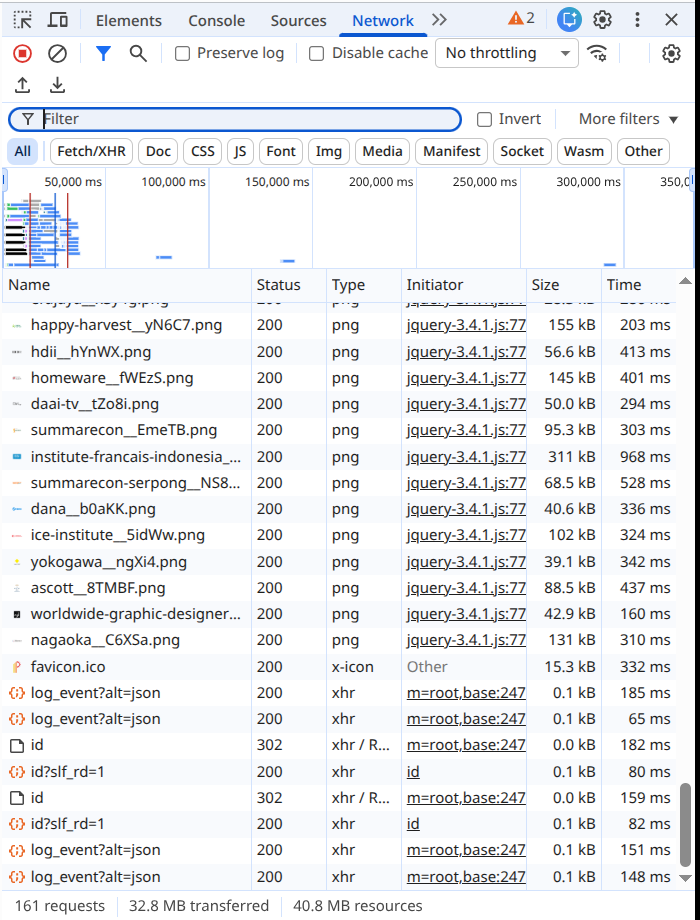
\includegraphics[width=0.72\textwidth, height=0.5\textheight,
                   keepaspectratio]{../figures/devtools-network.png}
  \caption{Panel Network pada Chrome DevTools saat memuat
           \texttt{www.pradita.ac.id}}
  \label{fig:devtools-network}
\end{figure}

\begin{enumerate}
  \item Buka jendela penyamaran, lalu tekan F12 untuk membuka DevTools dan
        pilih panel Network. Panel tersebut hanya merekam selama terbuka,
        sehingga langkah ini dilakukan sebelum halaman dimuat.
  \item Centang \emph{Disable cache} dan \emph{Preserve log}. Tanpa
        \emph{Disable cache}, sebagian besar aset tercatat 0 milidetik, karena
        diambil dari \textit{cache} browser dan tidak menyentuh jaringan sama
        sekali. Cirinya, kolom \emph{Size} menampilkan \emph{(memory cache)}
        atau \emph{(disk cache)}, bukan ukuran byte. Tanpa \emph{Preserve log},
        rekaman terhapus saat terjadi pengalihan, dan
        \texttt{pradita.ac.id} memang mengalihkan ke
        \texttt{www.pradita.ac.id}.
  \item Aktifkan kolom \emph{Protocol} dan \emph{Connection ID}. Kedua kolom
        ini tidak ditampilkan secara bawaan, sehingga harus dipasang sendiri.
        Arahkan penunjuk ke baris judul tabel permintaan, yaitu baris yang
        memuat tulisan \emph{Name}, \emph{Status}, \emph{Type},
        \emph{Initiator}, \emph{Size}, dan \emph{Time}. Klik kanan tepat pada
        baris tersebut, bukan pada baris permintaan di bawahnya, dan bukan pula
        pada bilah alat di atasnya. Menu yang muncul memuat seluruh kolom yang
        tersedia, lengkap dengan tanda centang pada kolom yang sedang aktif,
        seperti terlihat pada Gambar \ref{fig:menu-kolom}. Klik butir
        \emph{Protocol}, lalu ulangi klik kanan dan klik butir \emph{Connection
        ID}. Menu tertutup setiap kali satu butir dipilih, sehingga menyalakan
        dua kolom memang menuntut dua kali klik kanan.

\begin{figure}[!htb]
  \centering
  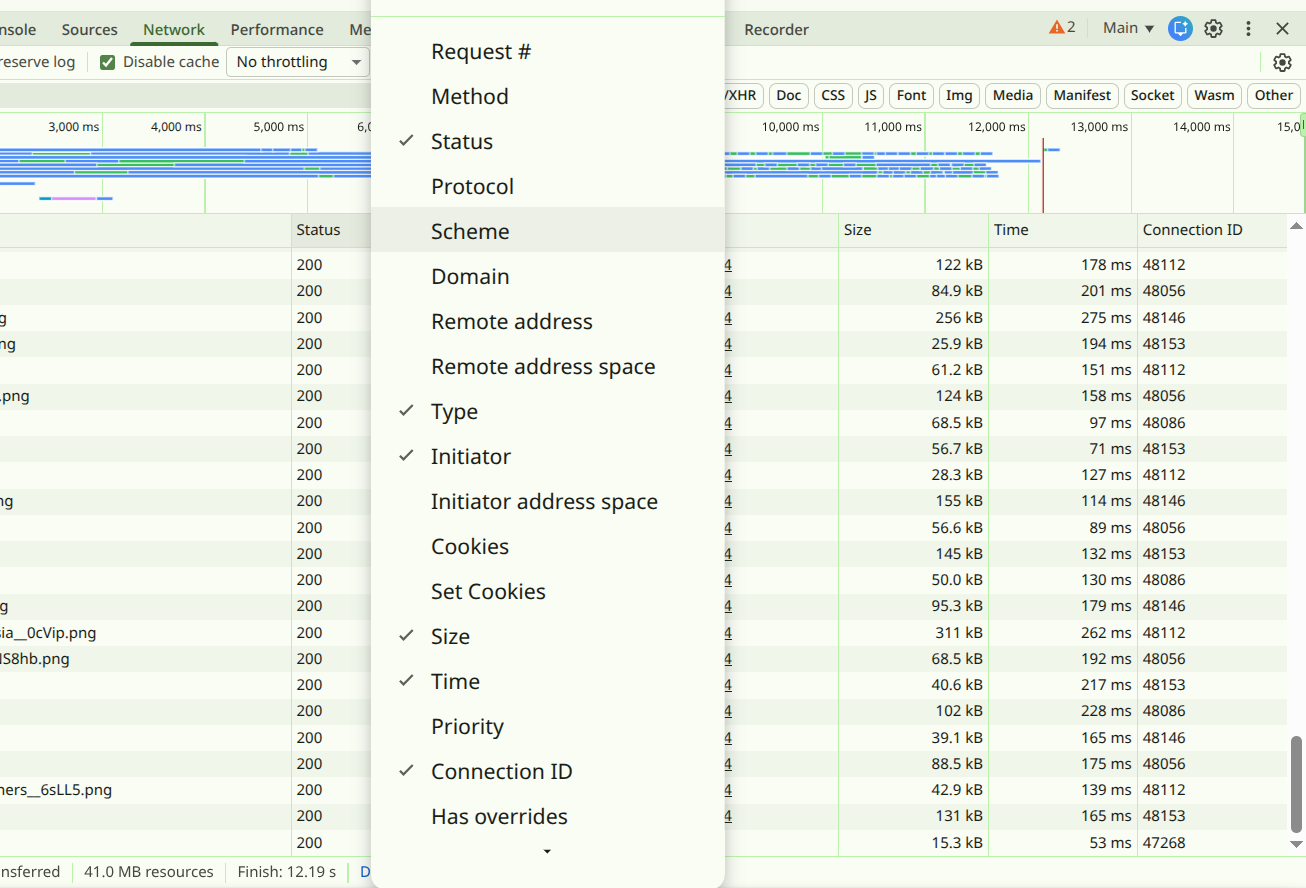
\includegraphics[width=0.68\textwidth, height=0.42\textheight,
                   keepaspectratio]{../figures/devtools-menu-kolom.png}
  \caption{Menu pemilihan kolom yang muncul setelah baris judul tabel
           permintaan diklik kanan. Butir \emph{Protocol} belum tercentang,
           sedangkan \emph{Connection ID} sudah}
  \label{fig:menu-kolom}
\end{figure}

  \item Setelah kedua kolom aktif, tabel permintaan menampilkan versi HTTP dan
        penanda koneksi untuk tiap aset, seperti pada Gambar
        \ref{fig:kolom-koneksi}. Nilai pada kolom \emph{Connection ID} adalah
        nomor soket yang dipakai permintaan tersebut. Nomor yang sama berarti
        permintaan berbagi satu koneksi, sedangkan nomor yang berbeda berarti
        koneksi terpisah. Pada gambar tersebut terlihat beberapa nomor berbeda,
        karena aset halaman berasal dari beberapa host sekaligus.

\begin{figure}[!htb]
  \centering
  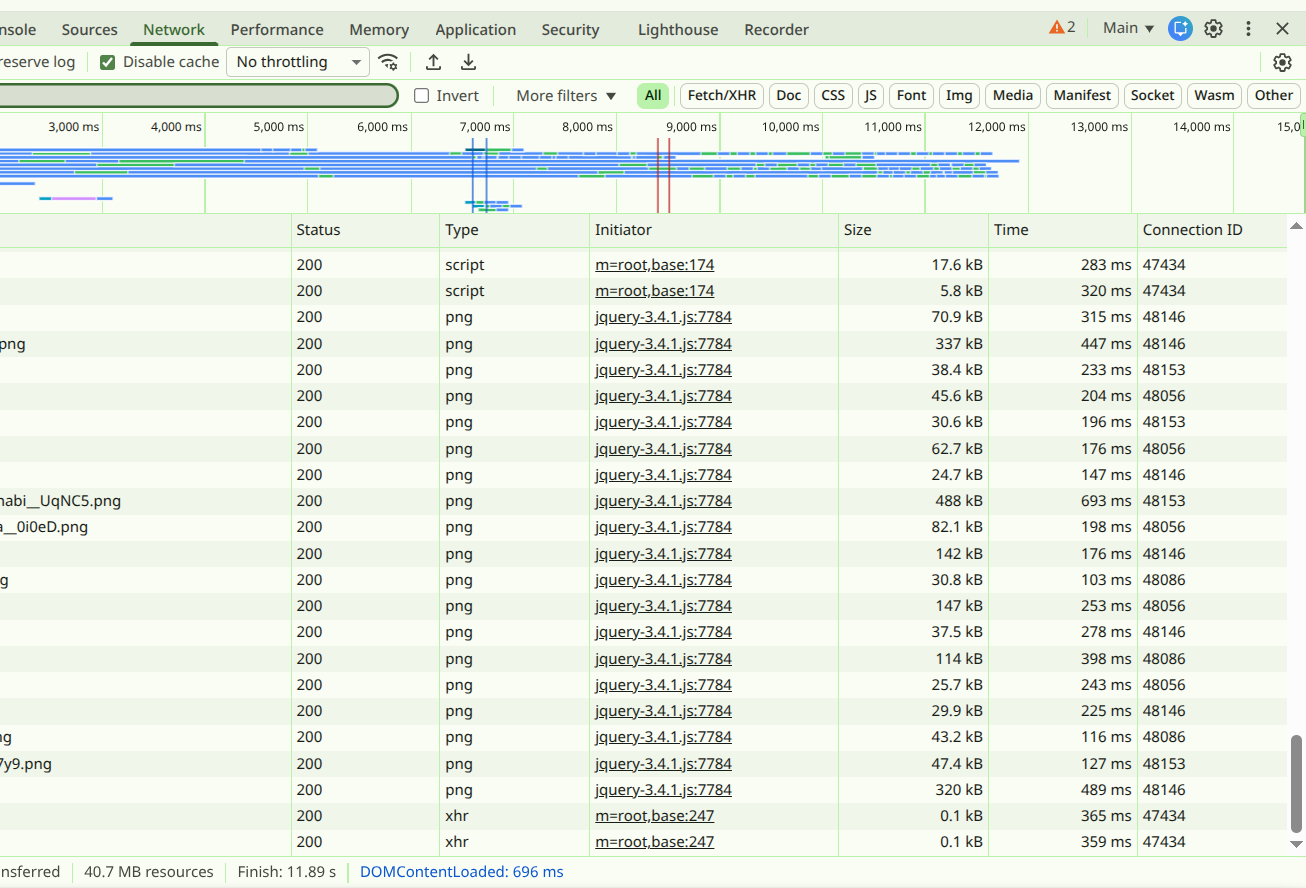
\includegraphics[width=0.68\textwidth, height=0.42\textheight,
                   keepaspectratio]{../figures/devtools-kolom-koneksi.png}
  \caption{Tabel permintaan setelah kolom \emph{Connection ID} diaktifkan.
           Nomor yang sama menandakan permintaan berbagi satu koneksi}
  \label{fig:kolom-koneksi}
\end{figure}

  \item Buka \texttt{aset.txt} yang dihasilkan skrip pada langkah sebelumnya.
        Berkas itu memuat lima alamat aset, misalnya
        \texttt{stylenew.css}, \texttt{stylenewcustom.css},
        \texttt{font-awesome.css}, \texttt{logo\_universitas.png}, dan
        \texttt{Web-Banner-Juli-2019.jpg}.
  \item Ketik nama salah satu berkas tersebut pada kotak filter di panel
        Network, misalnya \texttt{stylenew.css}. Daftar permintaan akan
        menyusut menjadi baris yang cocok saja. Catat nilai kolom
        \emph{Protocol} dan \emph{Connection ID} pada baris itu, lalu ulangi
        untuk kelima aset. Karena hanya lima, penghitungannya cukup manual.
  \item Isi baris browser pada Tabel \ref{tab:lat2-hasil} dari catatan
        tersebut. Protokolnya sama untuk kelima aset. Jumlah koneksi dihitung
        dari banyaknya nilai \emph{Connection ID} yang berbeda. Konkurensi
        dilihat dari kolom \emph{Waterfall}, yaitu berapa batang yang mulai
        pada waktu berdekatan. Waktu diambil dari ringkasan \emph{Finish} di
        bagian bawah panel.
  \item Perlu dicatat, pada browser konkurensi tidak dapat ditentukan sendiri.
        Browser yang memutuskan berapa permintaan berjalan bersamaan, dan
        keputusan itu dipengaruhi versi HTTP, prioritas aset, serta batas
        koneksi per host. Karena itu baris browser diisi dengan hasil
        pengamatan, bukan dengan skenario yang dipilih. Peran \texttt{curl}
        justru sebaliknya, yaitu memaksa skenario tertentu agar pengaruh tiap
        faktor dapat dipisahkan.
  \item Perlu dicatat pula, tanpa filter, jumlah permintaan pada browser jauh
        lebih banyak daripada lima aset tersebut. Browser juga memuat dokumen
        HTML-nya sendiri serta berkas yang baru ketahuan setelah CSS dan
        JavaScript dijalankan. Filter itulah yang menyamakan cakupan
        pengukuran browser dengan pengukuran \texttt{curl}.
  \item Jalankan perintah pada Listing \ref{lst:lat2-jalan}. Skrip tersebut
        mengumpulkan lima alamat aset halaman yang dituju ke
        \texttt{aset.txt}, memeriksa versi HTTP tiap host, lalu mengambil aset
        tersebut dalam empat skenario, yaitu berurutan tanpa pemakaian ulang
        koneksi, berurutan dengan \textit{keep-alive}, serentak di atas
        HTTP/1.1, dan serentak di atas HTTP/2. Secara bawaan hanya aset milik
        host halaman itu sendiri yang diambil. Jumlah koneksi diambil
        dari \texttt{\%\{num\_connects\}} milik \texttt{curl}, sedangkan pada
        browser angka itu terlihat dari banyaknya nilai berbeda pada kolom
        \emph{Connection ID}.
  \item Isi Tabel \ref{tab:lat2-hasil}. Tabel \ref{tab:lat2-contoh}
        memperlihatkan contoh hasilnya.
  \item Jawab tiga pertanyaan berikut. Pertama, mengapa skenario pertama
        memakai lima koneksi tetapi tetap paling lambat? Kedua, apa yang
        membedakan skenario ketiga dan keempat, padahal konkurensinya sama?
        Ketiga, mengapa jumlah aset tetap penting pada ketiga versi HTTP?
\end{enumerate}

Skrip tersebut memanggil \texttt{kumpulkan-aset.sh} yang juga tersedia pada
direktori yang sama. Jalankan dengan perintah pada Listing
\ref{lst:lat2-jalan}.

Kejadian 0 milidetik tersebut layak diperiksa lebih jauh, karena aset situs
kampus tidak mengirim header \texttt{Cache-Control} maupun \texttt{Expires}.
Yang dikirim hanya \texttt{Last-Modified} dan \texttt{ETag}, seperti terlihat
pada Listing \ref{lst:header-aset}. Dalam keadaan itu browser memakai
\textit{heuristic caching}, yaitu menebak masa berlaku dari umur berkas. Berkas
yang terakhir diubah lebih dari setahun lalu dianggap masih \textit{fresh} untuk waktu
yang lama, sehingga permintaan berikutnya dilayani dari \textit{cache} tanpa
menghubungi server. Perilaku ini dibahas lebih dalam pada bab \textit{caching},
dan untuk latihan ini cukup dimatikan lewat \emph{Disable cache}.

\begin{lstlisting}[language=bash, caption={Header aset situs kampus, tanpa \texttt{Cache-Control}}, label={lst:header-aset}]
curl -sI https://www.pradita.ac.id/assets/front/css/stylenew.css \
  | grep -iE "cache-control|expires|etag|last-modified"

# Keluarannya:
# last-modified: Fri, 14 Mar 2025 07:37:06 GMT
# etag: "67d3dca2-965"
\end{lstlisting}

\begin{lstlisting}[language=bash, caption={Menjalankan skrip pembanding pada aset milik situs kampus}, label={lst:lat2-jalan}]
cd sources/chapter02
./banding-http.sh https://www.pradita.ac.id/ 5

# Keluarannya:
# Host aset dan versi HTTP yang dilayaninya:
#   www.pradita.ac.id                    HTTP/2    5 aset
#
#   Skenario                            Konkurensi  Koneksi     Waktu
#   1. HTTP/1.1 berurutan, koneksi baru      1         5     2.14 detik
#   2. HTTP/1.1 berurutan, keep-alive        1         1     1.66 detik
#   3. HTTP/1.1 serentak                     5         5     1.92 detik
#   4. HTTP/2 serentak                       5         1     1.87 detik
\end{lstlisting}

\begin{table}[!htb]
  \centering
  \caption{Contoh hasil Latihan 3 yang sudah terisi, lima aset milik
           \texttt{www.pradita.ac.id}}
  \label{tab:lat2-contoh}
  \begin{tabularx}{\textwidth}{Xcccc}
    \hline
    \textbf{Skenario} & \textbf{Aset} & \textbf{Konkurensi} & \textbf{Koneksi} & \textbf{Waktu} \\
    \hline
    HTTP/1.1 berurutan, koneksi baru tiap aset & 5 & 1 & 5 & 2,14 detik \\
    \hline
    HTTP/1.1 berurutan, koneksi dipakai ulang & 5 & 1 & 1 & 1,66 detik \\
    \hline
    HTTP/1.1 serentak & 5 & 5 & 5 & 1,92 detik \\
    \hline
    HTTP/2 serentak & 5 & 5 & 1 & 1,87 detik \\
    \hline
  \end{tabularx}
\end{table}

Empat skenario pada Tabel \ref{tab:lat2-contoh} hanya dapat dipaksakan lewat
\texttt{curl}. Pada browser, keempatnya tidak dapat dipilih, karena browser
sendiri yang menentukan cara mengambil aset. Itulah sebabnya latihan ini memakai
dua alat: \texttt{curl} untuk memisahkan pengaruh tiap faktor, dan browser untuk
melihat perilaku yang sebenarnya terjadi.

Tabel \ref{tab:lat2-contoh} sengaja memisahkan dua hal yang sering tercampur.
Konkurensi berarti berapa permintaan berjalan bersamaan. Koneksi berarti berapa
saluran yang dibuka untuk mencapai konkurensi tersebut. Keduanya tidak selalu
seiring, dan itu terlihat jelas pada empat skenario tersebut.

Dua baris pertama sama-sama berurutan, yaitu permintaan berikutnya baru dikirim
setelah yang sebelumnya selesai. Bedanya hanya pada pemakaian ulang koneksi.
Baris pertama membuka koneksi baru untuk tiap aset, sehingga membayar DNS, TCP,
dan TLS lima kali. Baris kedua memakai satu koneksi untuk lima permintaan
berkat \textit{keep-alive}, dan waktunya turun. Perlu dicatat,
lima koneksi pada baris pertama dibuka bergantian, bukan bersamaan, sehingga
tidak dapat disebut paralel.

Dua baris terakhir barulah paralel, yaitu lima permintaan dikirim bersamaan.
Di sinilah perbedaan kedua versi terlihat. HTTP/1.1 mencapai paralelisme dengan
membuka lima koneksi, sedangkan HTTP/2 mencapainya di dalam satu koneksi lewat
\textit{multiplexing}. Hasil akhirnya mirip, tetapi biayanya berbeda.
Tiap koneksi tambahan menuntut rangkaian pembukaan sendiri dan memakan memori di
kedua sisi. Browser bahkan membatasi jumlahnya sekitar enam per host, sehingga
pada halaman dengan puluhan aset, sisanya harus mengantre.


Satu catatan soal pemilihan aset. Skrip \berkas{kumpulkan-aset.sh} secara
bawaan hanya mengambil aset yang dilayani host halaman itu sendiri. Halaman
kampus sebenarnya juga memuat aset dari domain lain, misalnya penyimpanan objek
dan CDN, dan sebagian di antaranya masih HTTP/1.1. Bila penyaringan tersebut
dimatikan dengan argumen \texttt{semua}, jumlah koneksi pada skenario keempat
akan naik, karena koneksi dihitung per host dan \textit{multiplexing} hanya
berlaku pada host yang mendukung HTTP/2. Hal itu sekaligus menunjukkan biaya
menyebar aset ke banyak domain, sebagaimana dibahas pada Seksi 2.3.
\begin{lstlisting}[language=bash, caption={Memeriksa dukungan HTTP/3 lewat header \texttt{alt-svc}}, label={lst:altsvc}]
curl -sI https://www.pradita.ac.id/ | grep -i alt-svc
# (tidak ada keluaran, berarti HTTP/3 belum diumumkan)

curl -sI https://www.google.com/ | grep -i alt-svc
# alt-svc: h3=":443"; ma=2592000,h3-29=":443"; ma=2592000
\end{lstlisting}


\begin{table}[!htb]
  \centering
  \caption{Lembar isian hasil pengukuran Latihan 3}
  \label{tab:lat2-hasil}
  \begin{tabularx}{\textwidth}{Xcccc}
    \hline
    \textbf{Skenario} & \textbf{Aset} & \textbf{Konkurensi} & \textbf{Koneksi} & \textbf{Waktu} \\
    \hline
    Browser, dibaca dari kolom \emph{Protocol} dan \emph{Connection ID} & 5 & \dots & \dots & \dots \\
    \hline
    HTTP/1.1 berurutan, koneksi baru tiap aset & 5 & 1 & \dots & \dots \\
    \hline
    HTTP/1.1 berurutan, koneksi dipakai ulang & 5 & 1 & \dots & \dots \\
    \hline
    HTTP/1.1 serentak & 5 & 5 & \dots & \dots \\
    \hline
    HTTP/2 serentak & 5 & 5 & \dots & \dots \\
    \hline
  \end{tabularx}
\end{table}

Pertanyaan berikutnya, mengapa HTTP/3 tidak ikut diukur. Ada dua alasan yang
keduanya dapat diperiksa sendiri. Pertama, \texttt{curl} bawaan Ubuntu tidak
dibangun dengan dukungan HTTP/3, sehingga opsi \texttt{--http3} ditolak dengan
pesan \emph{the installed libcurl version doesn't support this}. Dukungan itu
menuntut \texttt{libcurl} yang dibangun bersama pustaka QUIC seperti ngtcp2 atau
quiche, dan pembangunan tersebut di luar cakupan bab ini. Kedua,
\texttt{www.pradita.ac.id} sendiri belum menyediakan HTTP/3. Hal itu dapat
diperiksa tanpa mengunduh apa pun, yaitu lewat header \texttt{alt-svc} pada
respons, seperti pada Listing \ref{lst:altsvc}. Pada browser, versi yang
benar-benar dipakai terlihat pada kolom \emph{Protocol}, dengan nilai
\texttt{h2} untuk HTTP/2 dan \texttt{h3} untuk HTTP/3.



Angka waktu berubah tiap kali pengukuran dijalankan, karena bergantung pada
kondisi jaringan dan beban server. Yang perlu dilaporkan adalah pola
perbandingannya beserta penjelasannya, bukan angka persisnya.

